\section{Trigger\-Question Class Reference}
\label{classTriggerQuestion}\index{TriggerQuestion@{TriggerQuestion}}
Another Player-only {\bf Trigger}{\rm (p.\,\pageref{classTrigger})}, asking Yes/No question.  


{\tt \#include $<$triggerquestion.hpp$>$}

Inheritance diagram for Trigger\-Question::\begin{figure}[H]
\begin{center}
\leavevmode
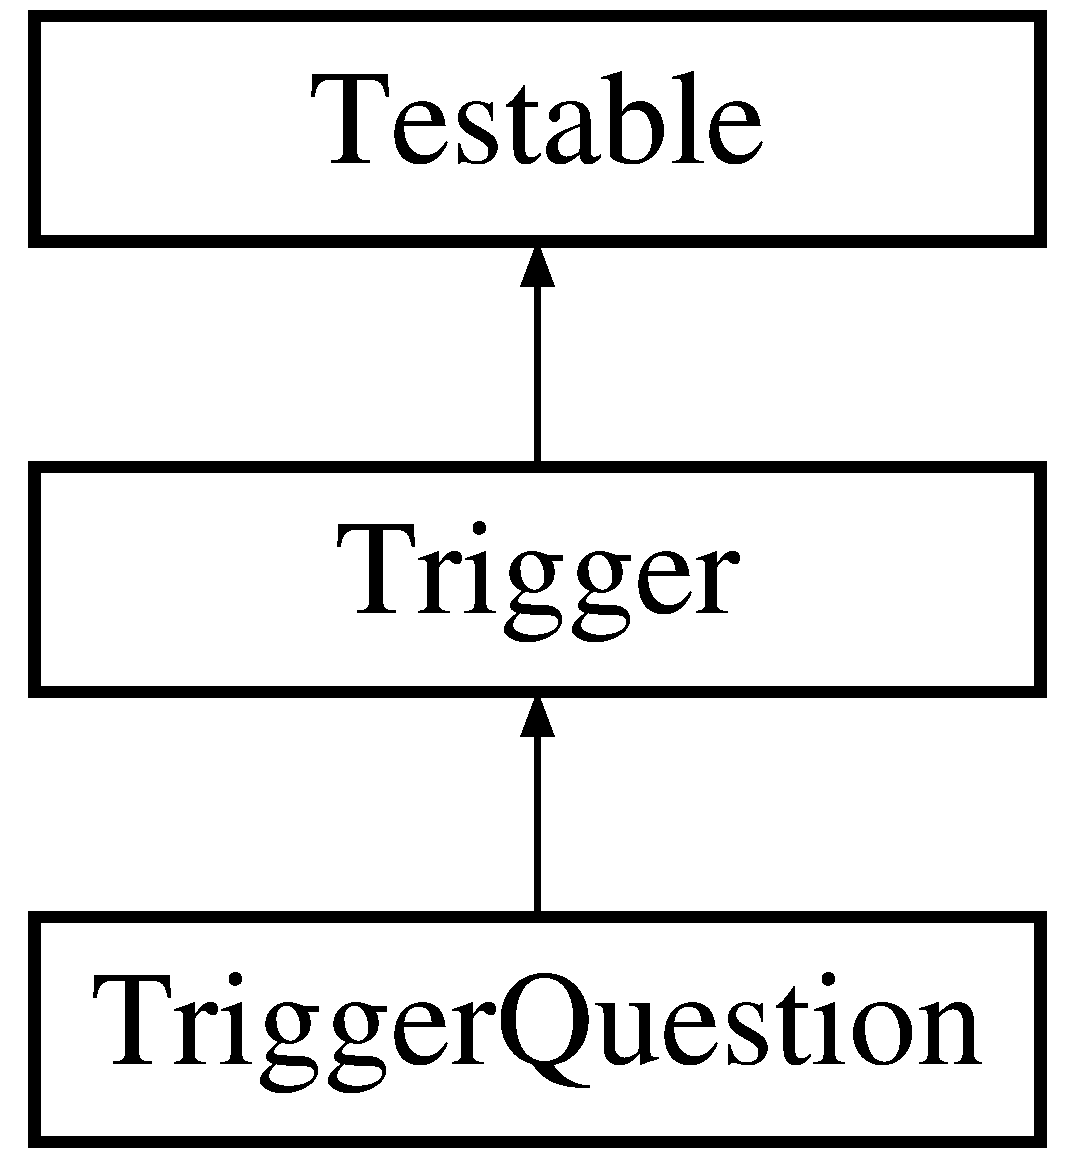
\includegraphics[height=3cm]{classTriggerQuestion}
\end{center}
\end{figure}
\subsection*{Public Member Functions}
\begin{CompactItemize}
\item 
{\bf Trigger\-Question} ()
\item 
{\bf $\sim$Trigger\-Question} ()
\item 
void {\bf cust\-Load} ({\bf Parser} \&parser)
\item 
void {\bf cust\-Save} (ofstream \&file) const 
\item 
bool {\bf can\-Activate} ({\bf Monster} \&monster)
\item 
QString {\bf name} () const 
\end{CompactItemize}
\subsection*{Public Attributes}
\begin{CompactItemize}
\item 
QString {\bf message}
\end{CompactItemize}


\subsection{Detailed Description}
Another Player-only {\bf Trigger}{\rm (p.\,\pageref{classTrigger})}, asking Yes/No question. 



\subsection{Constructor \& Destructor Documentation}
\index{TriggerQuestion@{Trigger\-Question}!TriggerQuestion@{TriggerQuestion}}
\index{TriggerQuestion@{TriggerQuestion}!TriggerQuestion@{Trigger\-Question}}
\subsubsection{\setlength{\rightskip}{0pt plus 5cm}{\bf Trigger\-Question} ()}\label{classTriggerQuestion_a0}


\index{TriggerQuestion@{Trigger\-Question}!~TriggerQuestion@{$\sim$TriggerQuestion}}
\index{~TriggerQuestion@{$\sim$TriggerQuestion}!TriggerQuestion@{Trigger\-Question}}
\subsubsection{\setlength{\rightskip}{0pt plus 5cm}$\sim${\bf Trigger\-Question} ()}\label{classTriggerQuestion_a1}




\subsection{Member Function Documentation}
\index{TriggerQuestion@{Trigger\-Question}!canActivate@{canActivate}}
\index{canActivate@{canActivate}!TriggerQuestion@{Trigger\-Question}}
\subsubsection{\setlength{\rightskip}{0pt plus 5cm}bool can\-Activate ({\bf Monster} \& {\em monster})\hspace{0.3cm}{\tt  [virtual]}}\label{classTriggerQuestion_a4}




Implements {\bf Trigger} {\rm (p.\,\pageref{classTrigger_a5})}.\index{TriggerQuestion@{Trigger\-Question}!custLoad@{custLoad}}
\index{custLoad@{custLoad}!TriggerQuestion@{Trigger\-Question}}
\subsubsection{\setlength{\rightskip}{0pt plus 5cm}void cust\-Load ({\bf Parser} \& {\em parser})\hspace{0.3cm}{\tt  [virtual]}}\label{classTriggerQuestion_a2}




Implements {\bf Trigger} {\rm (p.\,\pageref{classTrigger_b0})}.\index{TriggerQuestion@{Trigger\-Question}!custSave@{custSave}}
\index{custSave@{custSave}!TriggerQuestion@{Trigger\-Question}}
\subsubsection{\setlength{\rightskip}{0pt plus 5cm}void cust\-Save (ofstream \& {\em file}) const\hspace{0.3cm}{\tt  [virtual]}}\label{classTriggerQuestion_a3}




Implements {\bf Trigger} {\rm (p.\,\pageref{classTrigger_b1})}.\index{TriggerQuestion@{Trigger\-Question}!name@{name}}
\index{name@{name}!TriggerQuestion@{Trigger\-Question}}
\subsubsection{\setlength{\rightskip}{0pt plus 5cm}QString name () const\hspace{0.3cm}{\tt  [virtual]}}\label{classTriggerQuestion_a5}




Implements {\bf Trigger} {\rm (p.\,\pageref{classTrigger_a7})}.

\subsection{Member Data Documentation}
\index{TriggerQuestion@{Trigger\-Question}!message@{message}}
\index{message@{message}!TriggerQuestion@{Trigger\-Question}}
\subsubsection{\setlength{\rightskip}{0pt plus 5cm}QString {\bf message}}\label{classTriggerQuestion_o0}




The documentation for this class was generated from the following files:\begin{CompactItemize}
\item 
{\bf triggerquestion.hpp}\item 
{\bf triggerquestion.cpp}\end{CompactItemize}
